% !TEX TS-program = xelatex
% !TEX encoding = UTF-8
% !Mode:: "TeX:UTF-8"

\documentclass[onecolumn,oneside]{SUSTechHomework}

\usepackage{float}

\author{胡玉斌}
\sid{11712121}

\title{Lab 8}
\coursecode{CS315}
\coursename{Computer Security}

\begin{document}
\maketitle

\section*{Task 1}

We run the attack.py many times, and find if those information appear in the content. And we caught them all.

\subsection*{User name and password}

\begin{figure}[H]
  \centering
  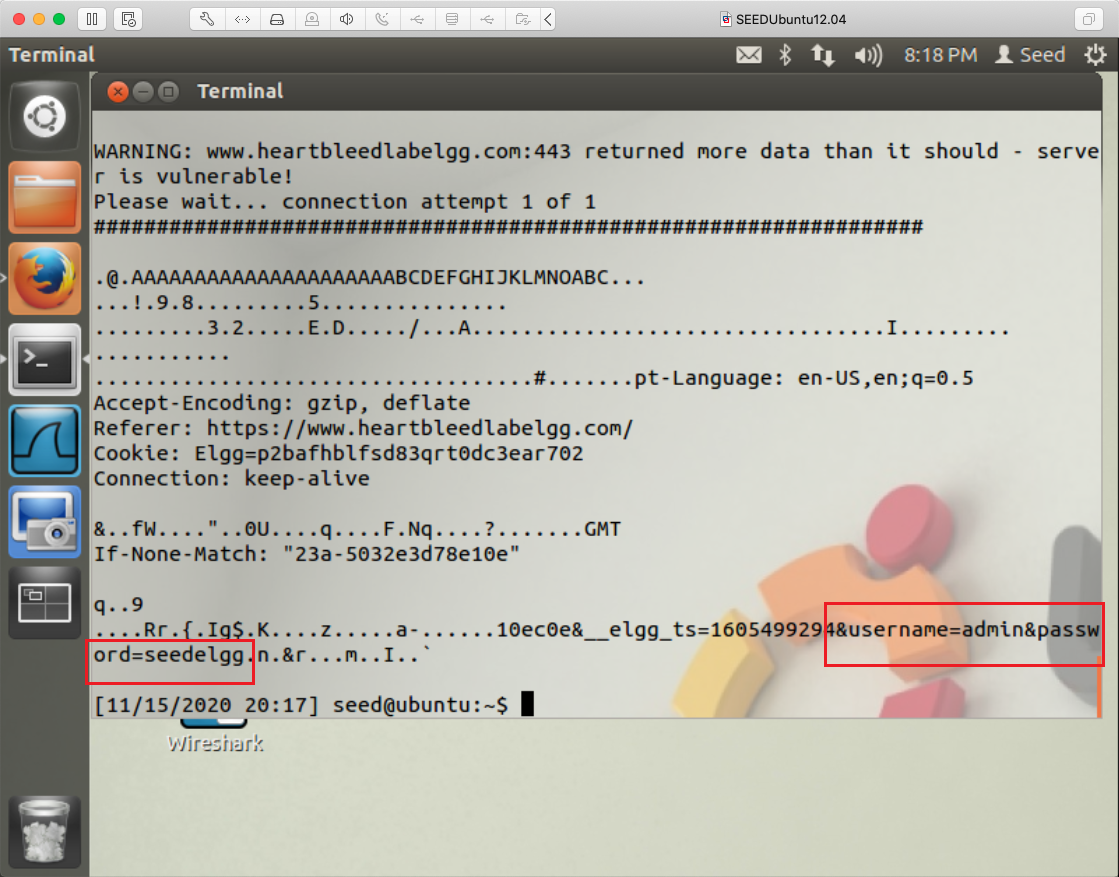
\includegraphics[width=0.85\textwidth]{img/p1.png}
  \caption{User name and password}
\end{figure}

\subsection*{User's acctivity}

\begin{figure}[H]
  \centering
  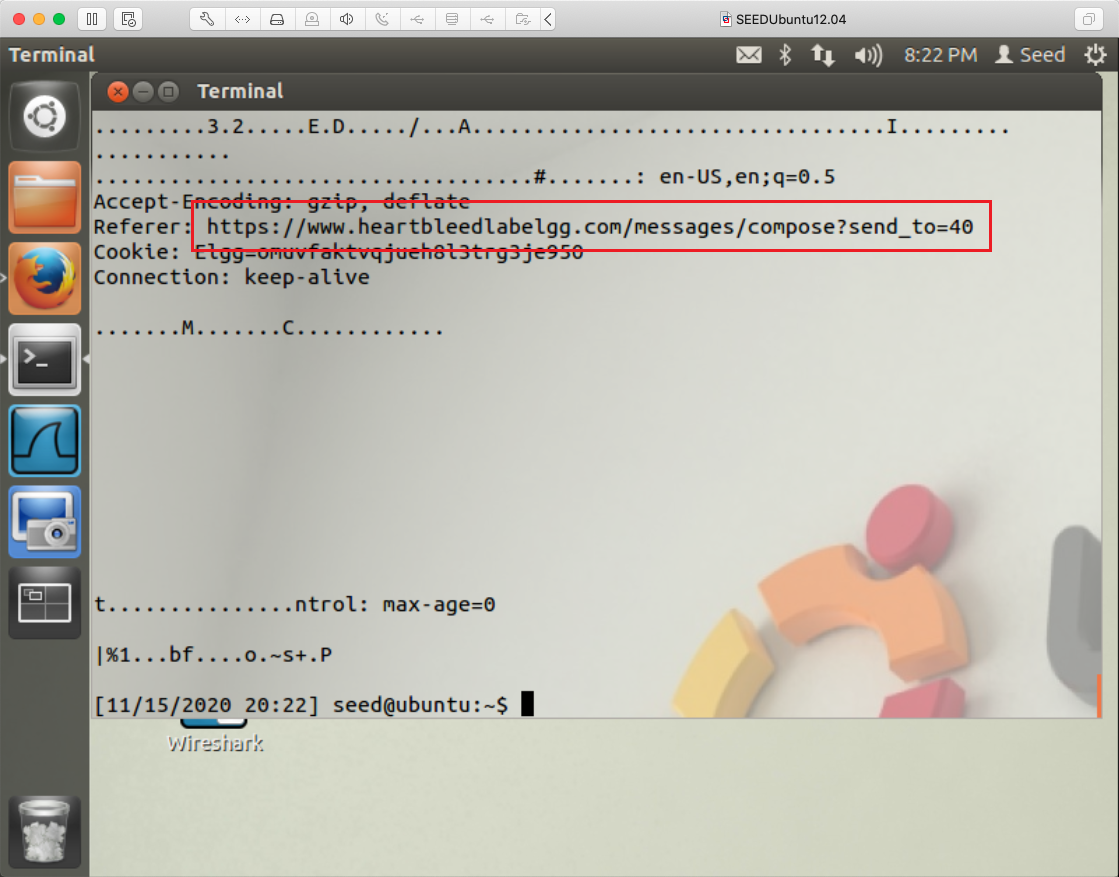
\includegraphics[width=0.85\textwidth]{img/p2.png}
  \caption{activity}
\end{figure}

\subsection*{message}

\begin{figure}[H]
  \centering
  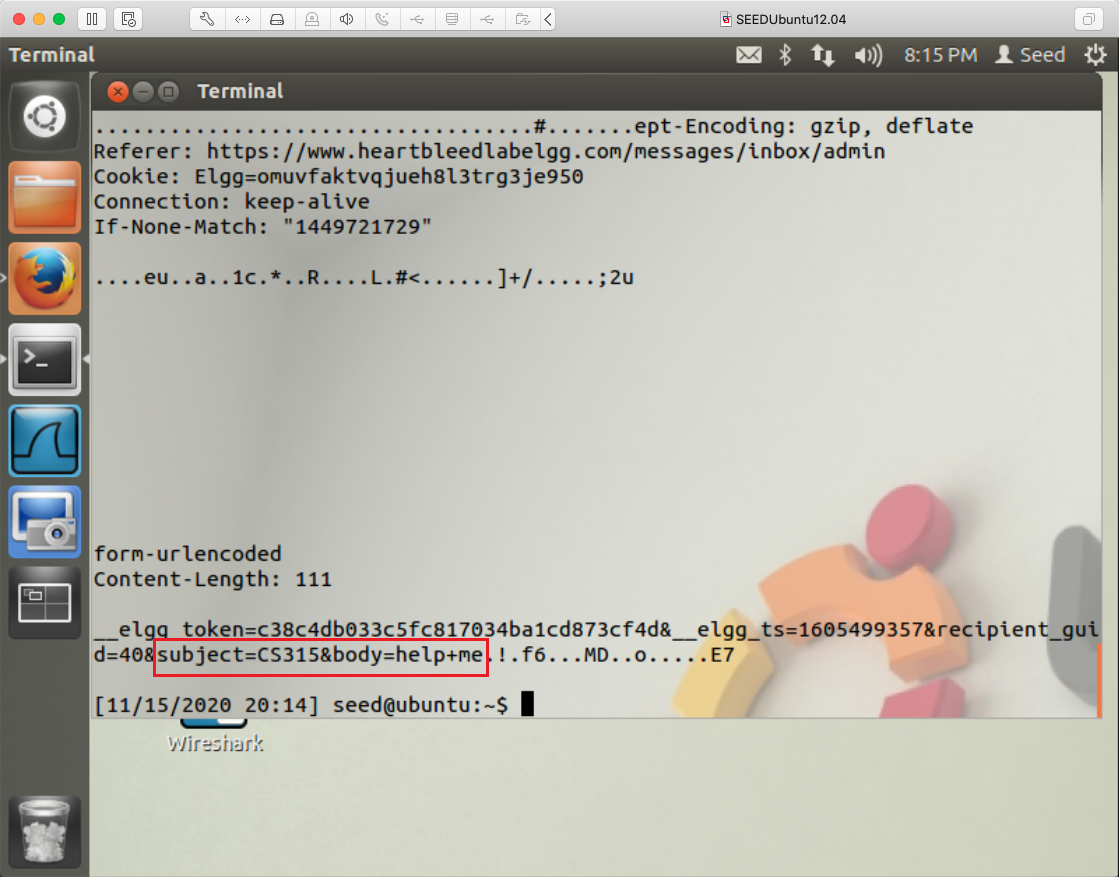
\includegraphics[width=0.85\textwidth]{img/p3.png}
  \caption{message}
\end{figure}

\section*{Task 2}

\subsection*{Question2.1}

As the length decreases, the length of content decreases.

\begin{figure}[H]
  \centering
  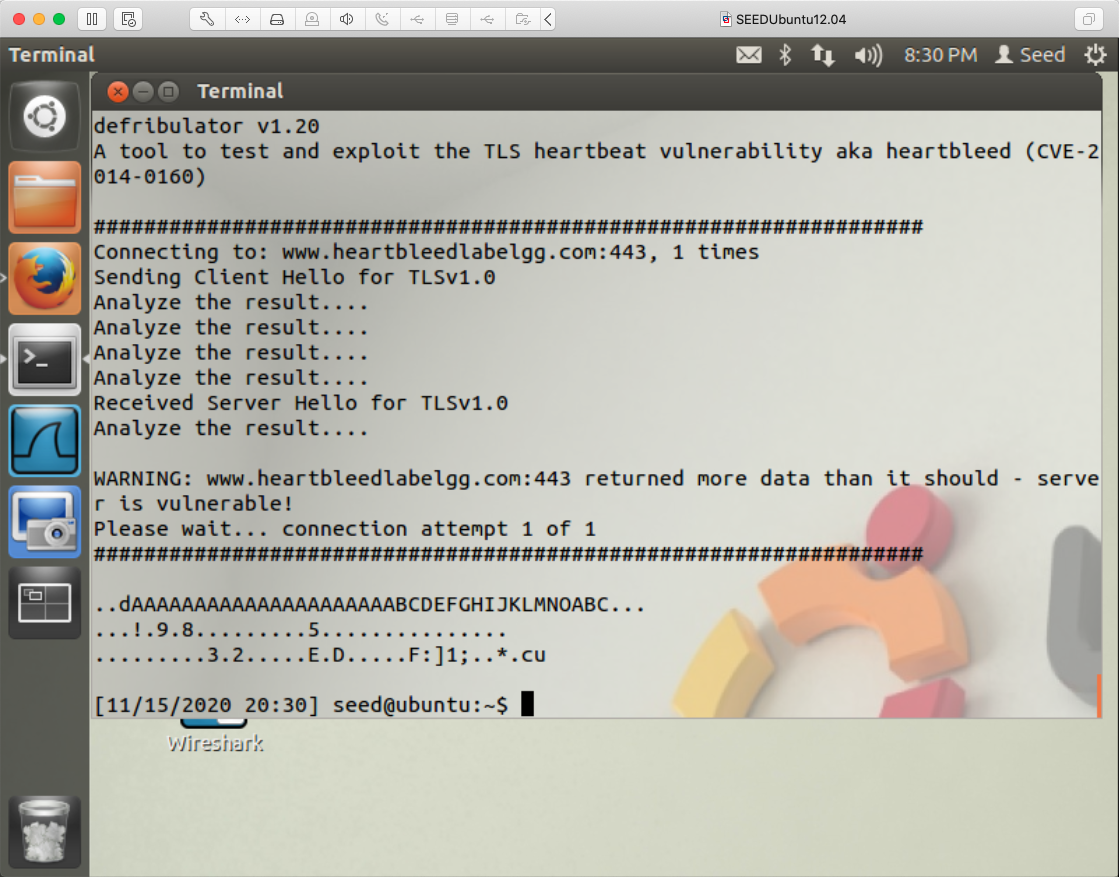
\includegraphics[width=0.85\textwidth]{img/p5.png}
  \caption{-l 50}
\end{figure}

\begin{figure}[H]
  \centering
  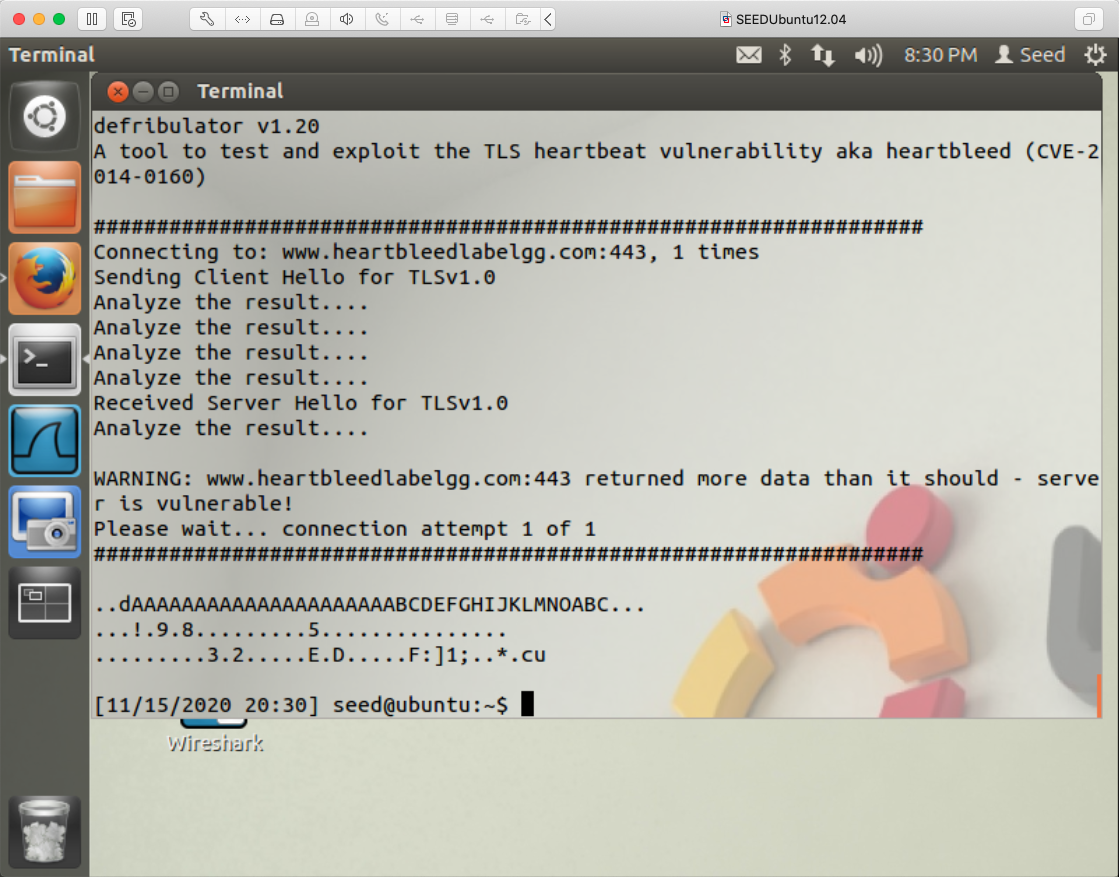
\includegraphics[width=0.85\textwidth]{img/p5.png}
  \caption{-l 100}
\end{figure}

\subsection*{Question2.2}

Server processed malformed Heartbeat, but did not return any extra data.

\begin{figure}[H]
  \centering
  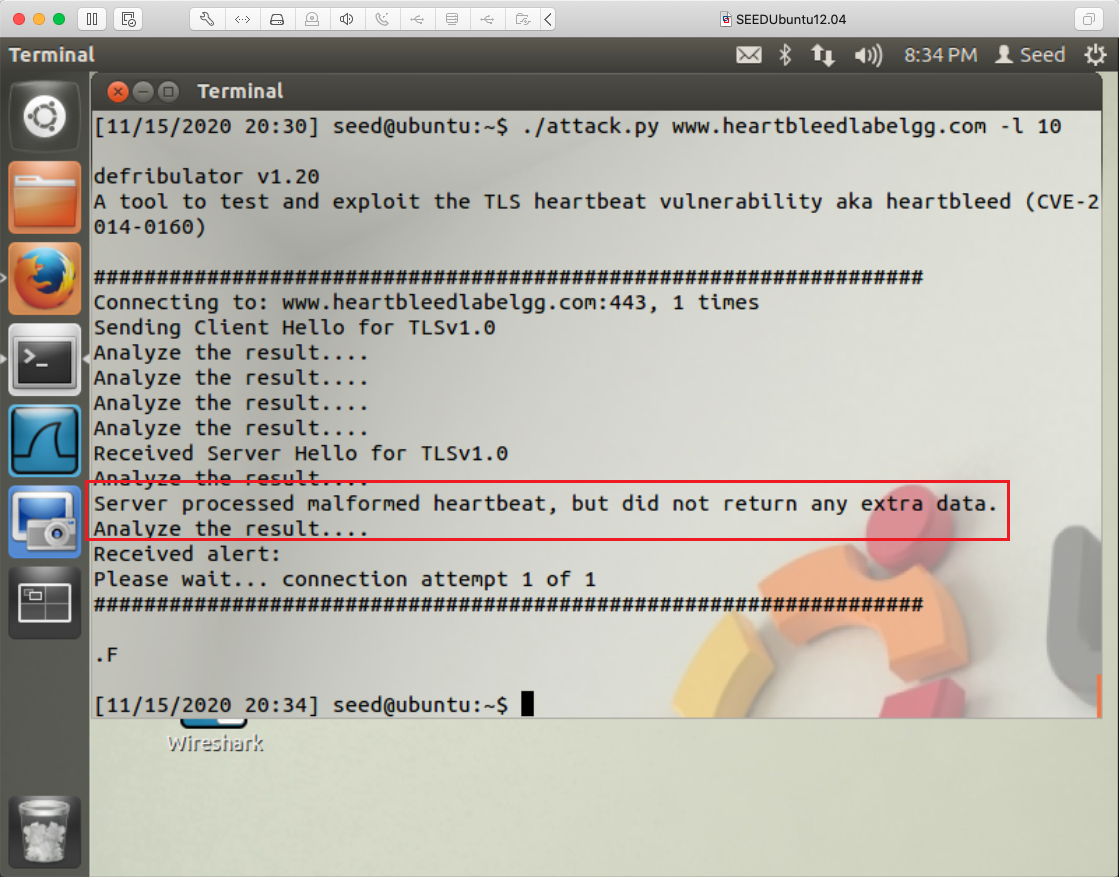
\includegraphics[width=0.85\textwidth]{img/p6.png}
  \caption{-l 10}
\end{figure}

\begin{figure}[H]
  \centering
  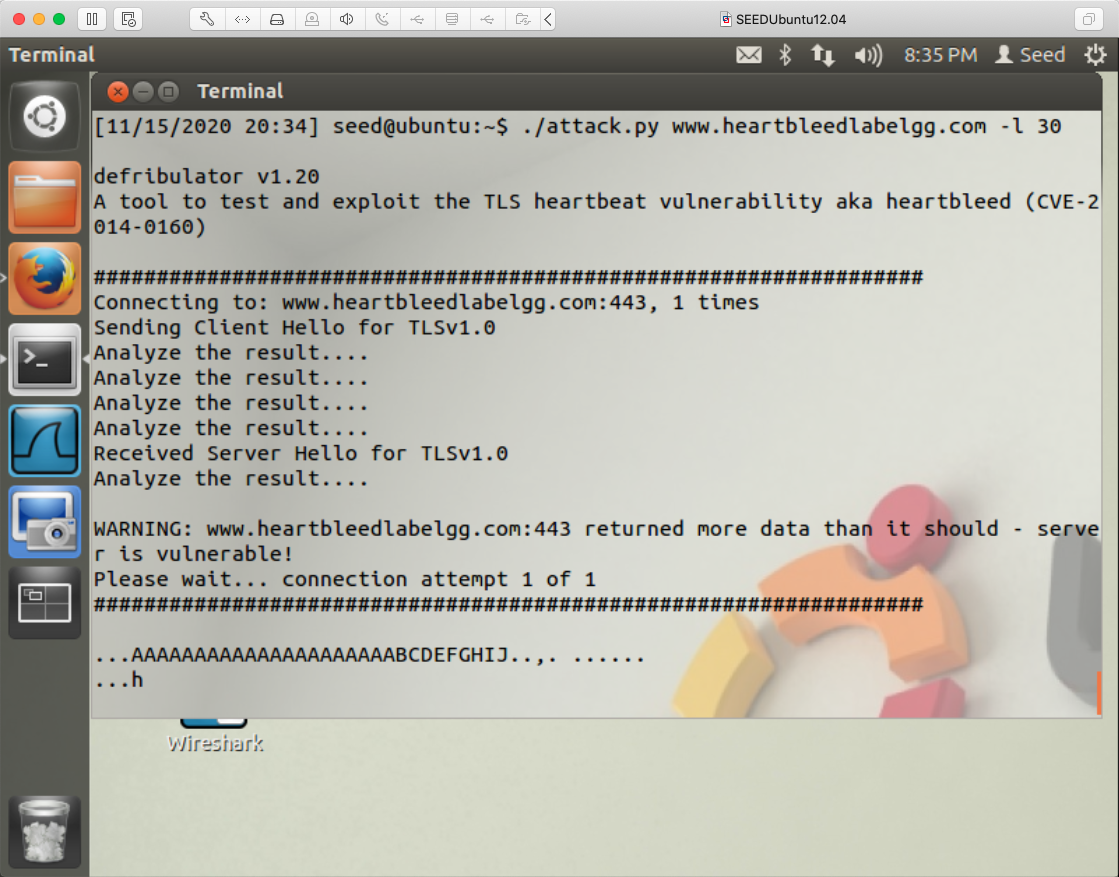
\includegraphics[width=0.85\textwidth]{img/p7.png}
  \caption{-l 30}
\end{figure}

\section*{Task 3}

\subsection*{Task3.1}

After we update the OpenSSL, the heartbleed attack cannot work.

\begin{figure}[H]
  \centering
  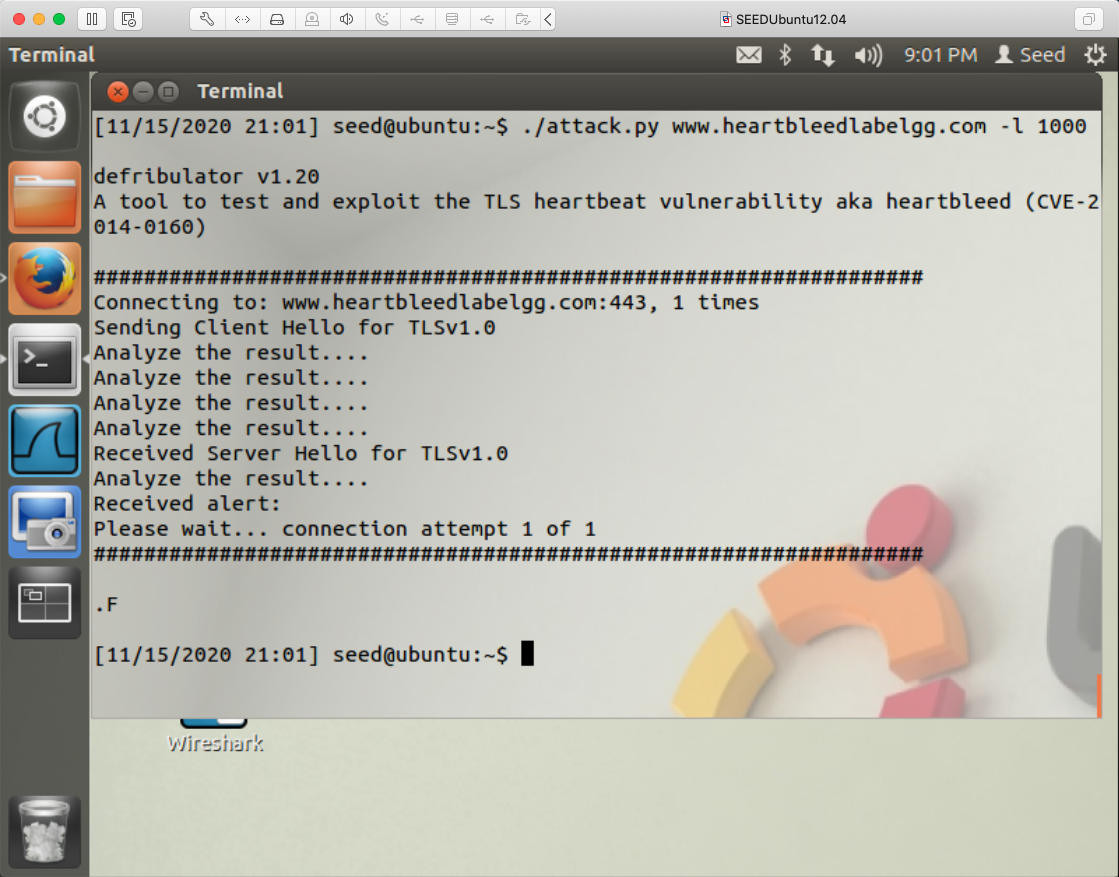
\includegraphics[width=0.85\textwidth]{img/p8.png}
  \caption{update}
\end{figure}

\subsection*{Task3.2}

The solution to fix this bug is counting the length of the payload field in the package, then check the payloud\_length cannot trigger the heartbleed attack.

Comment: Bob's idea is correct. The cause of this volnerability is lack of input validation not boundary check. The length filed cannot be removed because it is part of heartbleed protocol.

\section*{Task 4}

\end{document}
